\newpage
\section{Vorbereitung}
Lesen Sie die Wikipedia-Einträge über
\begin{itemize}
	\item Hardware Abstraction [\url{http://en.wikipedia.org/wiki/Hardware\_abstraction}],
	\item Logikpegel $"$High-Active$"$ und $"$Low-Active$"$ [\url{https://de.wikipedia.org/wiki/Logikpegel}],
	\item Prellen [\url{http://de.wikipedia.org/wiki/Prellen}],
	\item Polling in der Informatik [\url{http://de.wikipedia.org/wiki/Pollin\_(Informatik)}] und
	\item Interrupts [\url{http://de.wikipedia.org/wiki/Interrupt}] nach.\\
\end{itemize}
Lesen Sie ferner, wie mittels der Energia-Bibliothek Interrupts [\url{http://energia.nu/AttachInterrupt.html}] verwendet werden.\\ \\
Sehen Sie Sich die Handhabung der Funkionen \textit{pinMode}, \textit{digitalWrite}, \textit{digitalRead} sowie die das Übertragen von Debugging Informationen mittels der \textit{Serial} Klasse in der Energia-Umgebung an.\\ \\
\section{Praktikum}
Speichern Sie das Listing 1 \textit{button\_loop.ino} (hinterlegt in ILIAS) lokal ab. Das Listing 1 enthält nur einen Teil eines Programms, das eine blinkende LED mittels eines Knopfdrucks auf den Taster ausschalten (Not-Aus) soll.\\ \\
Schlie\ss{}en Sie das LaunchPad über die Pins PC4, GND, +3.3V an das Steckbrett gemä\ss{} Schaltbild 1 an (mit 10 kOhm Widerstand).\\ \\
Welche Art der Beschaltung wurde für den Taster verwendet (Pull-Up oder Pull-Down und
High-Active oder Low-Active)?\\ \\
Es wurde ein Pull-Down-Widerstand verwendet (Der Widerstand ist zwischen PC4 und GND geschaltet). Der Taster hat zwei Zustände $"$nicht gedrückt$"$ und $"$gedrückt$"$. Wenn der Taster nicht gedrückt wird ist am Pin PC4 ein Low-Pegel. Wenn der Taster gedrückt wird ist am Pin PC4 ein High-Pegel. Ein High-Pegel stellt eine 0 dar und der Low-Pegel eine 1 dar. Das hei\ss{}t der Taster ist low-aktiv.\\ \\
\begin{figure}[h]
\centering
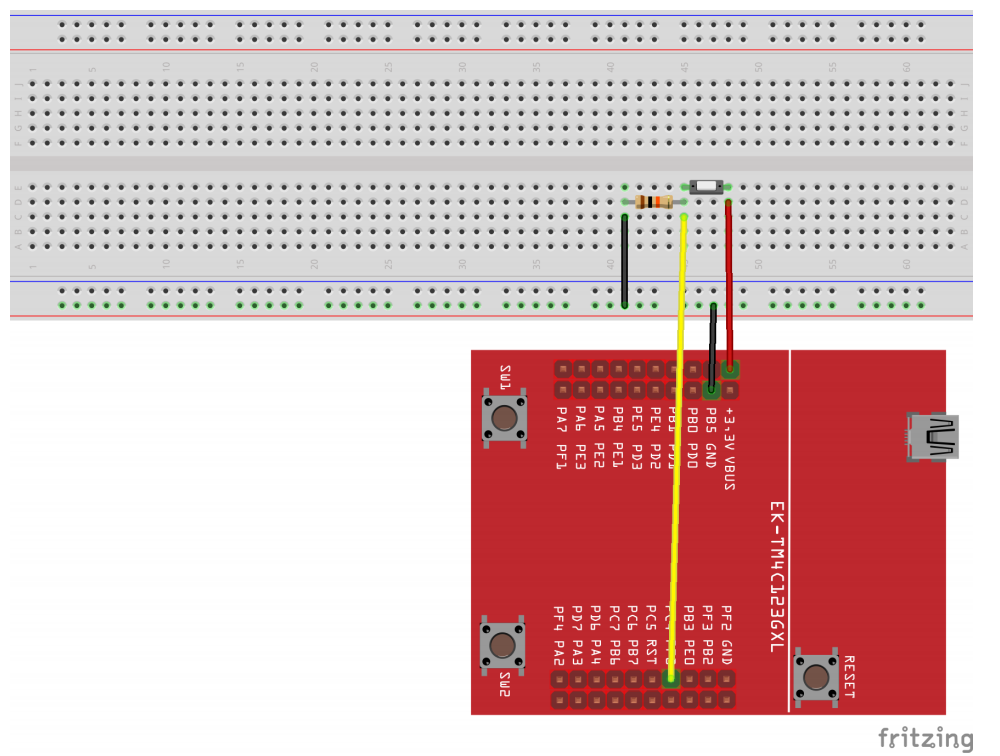
\includegraphics[width=0.7\linewidth]{images/Schaltbild1}
\caption{Schaltbild 1}
\label{fig:Schaltbild1}
\end{figure}
\newpage
\section{Aufgabe 1}
Implementieren Sie die fehlende Klasse \textit{TButton} (Konstruktor und Funktion \textit{state}).\\ \\
Laden Sie das Programm auf das LaunchPad hoch und testen Sie es. (Tipp: Das\\
Programm können Sie mit dem Knopf „Reset“ auf dem LaunchPad neustarten.)\\ \\
Wie verhält sich ein Auslösen des $“$Not-Aus-Knopfs$”$ hinsichtlich der Reaktionszeit?\\
\begin{lstlisting}[label =lst:bash]
template <const uint8_t PORT_NB>
class TButton {
  public:
    TButton(const uint8_t f_btnState = LOW)
      : m_btnState(f_btnState) {
      pinMode(PORT_NB, INPUT);
    }
    uint8_t state() {
      m_btnState = digitalRead(PORT_NB);
      return m_btnState;
    }
  private:
  uint8_t m_btnState;
};
\end{lstlisting}
Der Not-Aus-Knopf reagiert nach dem er ein Paar Sekunden gedrückt wurde.
\newpage
\section{Aufgabe 2}
Verbessern Sie das Programm hinsichtlich der Reaktionszeit, indem Sie Polling einsetzen.\\
\begin{lstlisting}[label =lst:bash]
unsigned long time1, time2, time;
void setup() {
  Serial.begin(9600);
}

void loop() {
  Serial.println("Start");  
  if(Button.state() == HIGH) {
    time1 = micros();
    Led.off();
    time2 = micros();
    time = time2 - time1;
    Serial.println(time);
  } else {
    Led.toggle(); 
  }
  delay(Delay);   
}
\end{lstlisting}
Die Methode loop() wird zyklisch aufgerufen dementsprechend wird die state Methode zyklisch aufgerufen..\\
\section{Aufgabe 3}
Geben Sie mittels der Serial-Klasse Debug-Informationen vom LaunchPad an Ihr System\\
aus, wenn der Not-Aus-Knopf betätigt wird.\\ \\
Mit der Methode Serial.begin(int) wird die Ausgabe der Debug-Informationen begonnen bzw. vorbereitet. Mit der Methode Serial.println(val) wird eine Zeile ausgegeben.\\ \\
\newpage
\section{Aufgabe 4}
Implementieren Sie nun die Not-Aus-Funktionalität mittels Nutzung der TivaWare-ROM-\\
Funktionen zur Auslösung eines Interrupts, d.h. ohne Energia-Funktion attachInterrupt()\\
zu benutzen. Schreiben Sie hierzu ein neues Programm.\\
(Siehe TivaWare™ Peripheral Driver Library. Dazu könnten Ihnen auch Lab3 und Lab4\\
des LaunchPad-Workbooks helfen.)\\ \\
\begin{lstlisting}[label =lst:bash]
void IntHandler(void);

// global instances for led output
TLed<LedPortOut> Led;
// and for button pin 
TButton<ButtonPinIn> Button;

void setup() {
	IntRegister(INT_UART0, IntHandler);
	IntEnable(INT_UART0);
	IntMasterEnable();
}

void loop() {
	if(Button.state() == LOW) { 
		Led.toggle(); 
	}
	delay(Delay);
}

void IntHandler(void) {
	if(Button.state() == HIGH) {
	Led.off();
	} 
}
\end{lstlisting}
Die Methode IntRegister(INT\_UART0, IntHandler) registriert die Methode IntHandler(). Die wird aufgerufen wenn ein Interrupt (UART 0) ein tritt.\\
Die Methode IntEnable(INT\_UART0) aktiviert den UART O Interupt beim Interupt-Controller.\\
Die Methode IntMasterEnable() erlaubt dem Prozessor auf dem Interupt zu antworten.\\ \\
\newpage
\section{Aufgabe 5}
Schreiben Sie nun ein weiteres Programm, das die LED des LaunchPads über den Taster\\
an- bzw. ausschaltet (toggeln). Stellen Sie dabei sicher, dass Ihre Implementierung\\
der Klasse TButton eine Entprellung des Tasters vornimmt.\\ \\
\begin{lstlisting}[label =lst:bash]
void off() {
	if(m_disabled == false) {
		m_disabled = true; 
		m_ledState = LOW;
		// set led to current state      
		digitalWrite(PORT_NB, m_ledState);
	} 
	else {
		m_disabled = false;
		m_ledState = HIGH;
		// set led to current state      
		digitalWrite(PORT_NB, m_ledState);
	}
}
\end{lstlisting}
	